\documentclass[conference]{IEEEtran}
\usepackage{ifpdf}
\usepackage{booktabs}
\usepackage{cite}
\usepackage[cmex10]{amsmath}
\usepackage{amsfonts}
\usepackage{url}
\usepackage{color}
\usepackage[utf8]{inputenc}
\usepackage{algpseudocode}
\usepackage{algorithm}
\usepackage{booktabs}
\usepackage{tabularx}
\usepackage{multicol}
\usepackage{bm}
\usepackage{multirow}
\usepackage{array}
\usepackage{epstopdf}
\usepackage{siunitx}
\ifCLASSINFOpdf
   \usepackage[pdftex]{graphicx}
  % declare the path(s) where your graphic files are
   \graphicspath{{figures/png/}}
  % and their extensions so you won't have to specify these with
  % every instance of \includegraphics
  \DeclareGraphicsExtensions{.png}
\else
  % or other class option (dvipsone, dvipdf, if not using dvips). graphicx
  % will default to the driver specified in the system graphics.cfg if no
  % driver is specified.
  \usepackage[dvips]{graphicx}
  % declare the path(s) where your graphic files are
  \graphicspath{{figures/eps/}}
  % and their extensions so you won't have to specify these with
  % every instance of \includegraphics
  \DeclareGraphicsExtensions{.eps}
\fi
\usepackage{epsfig}
\newcolumntype{M}{>{$\vcenter\bgroup\hbox\bgroup}c<{\egroup\egroup$}}
\newcommand{\etal}{\textit{et al.}}

\DeclareMathOperator*{\argmin}{argmin}
\newcommand\undermat[2]{%
	\makebox[0pt][l]{$\smash{\underbrace{\phantom{%
					\begin{matrix}#2 \end{matrix}}}_{\text{$#1$}}}$}#2}
\usepackage[font=small, labelfont=bf, format=plain, labelsep=space, figurename=Figure, tablename=Table]{caption}\usepackage[labelfont=rm, labelformat=parens, labelsep=space]{subcaption}

\begin{document}
%
% paper title
% Titles are generally capitalized except for words such as a, an, and, as,
% at, but, by, for, in, nor, of, on, or, the, to and up, which are usually
% not capitalized unless they are the first or last word of the title.
% Linebreaks \\ can be used within to get better formatting as desired.
% Do not put math or special symbols in the title.
\title{A compressed beamforming framework for ultrafast ultrasound imaging}

\author{\IEEEauthorblockN{Adrien Besson\IEEEauthorrefmark{1},
Rafael E. Carrillo\IEEEauthorrefmark{1}, 
Dimitris Perdios\IEEEauthorrefmark{1},
Marcel Arditi\IEEEauthorrefmark{1},
Olivier Bernard\IEEEauthorrefmark{2},
Yves Wiaux\IEEEauthorrefmark{3},} and 
Jean-Philippe Thiran\IEEEauthorrefmark{1}\IEEEauthorrefmark{4}
\IEEEauthorblockA{\IEEEauthorrefmark{1}Signal Processing Laboratory (LTS5),
Ecole Polytechnique F\'{e}d\'{e}rale de Lausanne,
Lausanne, Switzerland\\}
\IEEEauthorblockA{\IEEEauthorrefmark{2}CREATIS, CNRS UMR5220, University of Lyon, INSA-Lyon, University of Lyon1, Villeurbanne, France}
\IEEEauthorblockA{\IEEEauthorrefmark{3}Institute of Sensors, Signals and Systems, Heriot-Watt University, Edinburgh, UK\\}
\IEEEauthorblockA{\IEEEauthorrefmark{4}Department of Radiology, University Hospital Center (CHUV) and University of Lausanne (UNIL), Lausanne, Switzerland}}
\maketitle

\begin{abstract}
Classical beamforming methods, based on Delay-And-Sum (DAS) require an extensive number of samples and  delay calculations to obtain high-quality images. Compressed Beamforming (CB) proposes an alternative to DAS, based on compressed sensing, which aims at reducing the data rate. However, proposed CB approaches induce a computationally heavy measurement model that hampers their attractiveness for iterative image reconstruction. In this paper, a CB framework, applicable to either radio-frequency or in-phase quadrature data and for both plane wave and diverging wave compounding, is described. The proposed framework exploits a computationally light measurement model which leads to tractable reconstruction. It solves a convex problem and assumes sparsity in a wavelet-based model to achieve high-quality image reconstruction from measurements acquired with only few transducer elements. 
\end{abstract}

\begin{IEEEkeywords}
Plane wave, Diverging wave, Ultrafast imaging, Sparsity, Compressed sensing, Beamforming
\end{IEEEkeywords}

\IEEEpeerreviewmaketitle

\section{Introduction}
\par Compressed-sensing based beamforming, also denoted as Compressed Beamforming (CB) relies on a Compressed Sensing (CS) framework~\cite{Candes_SPM_2008} to achieve data rate reduction as it has been successfully applied to other medical imaging modalities such as Magnetic Resonance Imaging (MRI)~\cite{Lutsig_MRM_2007}. In order to apply CS onto an imaging problem, the image reconstruction process has to be formulated as an inverse problem and the unknown desired image has to be compressible \textit{i.e} sparse in a given model. Based on these two assumptions, the desired image is retrieved by solving a convex optimization problem. 
\par In ultrasound (US) imaging, CS has been extensively used for various purposes. Liebgott \etal{}~\cite{Liebgott_Ult_2013} use the sparsity of backscattered echoes in the wave atom frame to reduce the number of required echoes in a pre-beamforming step.  The objective of such an approach is to reduce the complexity of the probe hardware by simplifying cabling. In a post-beamforming step, CS has been used for two main purposes, namely data rate reduction and image quality enhancement through deconvolution~\cite{Chen2015}. A sparsity prior of Radio-Frequency~(RF) images has been exploited in various models such as: Fourier basis~\cite{Quinsac2012}, wavelet basis~\cite{Quinsac2012}, $\alpha-$stable distribution~\cite{Dobigeon2012} or more recently in learned dictionaries~\cite{Lorintiu_TMI_2015}. Finally, CB has been used as an alternative to classical beamforming methods. Schiffner and Schmitz~\cite{Schiffner_IUS_2012} introduced plane-wave-based CS beamforming in which the inverse scattering problem is solved in the time-frequency domain. Recently, David \etal{}~\cite{David_JASA_2015} introduced a simplified model in which the inverse scattering problem is solved only in the time domain. Fourier-based CS beamforming has also been studied by Chernyakova \etal{}~\cite{Chernyakova2014} in which a finite rate of innovation framework is used to reduce the data rate while the beamforming is achieved in the Fourier domain.
\par The main problem of CS based beamforming is the size of the measurement model, usually prohibitive~\cite{Schiffner_IUS_2012}, which prevents its use in US imaging. In this paper, we formulate the inverse problem using a simplified measurement model that can be stored as a sparse matrix. Such a measurement model allows fast reconstructions using iterative algorithms. The inverse problem is applicable to any type of transmit scheme but the present study focuses on coherent Plane Wave (PW) and Diverging Wave (DW) compounding. The proposed model is expressed for both RF and In-phase Quadrature (IQ) images.
\par Section \ref{sec:CS} briefly reviews CS principles. The compressed beamforming framework is then described in Section \ref{sec:CB}. Finally, the proposed framework is evaluated through simulation and \textit{in vivo} experiments in Section \ref{sec:exp} and concluding remarks are given in Section \ref{sec:Conc}.
\section{Principles of compressed sensing}
\label{sec:CS}
The now famous theory of CS introduces a signal acquisition framework that goes beyond the traditional Nyquist sampling paradigm\cite{fornasier11}.
Formally, the signal $\bm{x} \in \mathbb{C}^N$ is acquired through the linear measurement model $\mathsf{\Phi} \in \mathbb{C}^{M \times N}$ and $\bm{y} = \mathsf{\Phi} \bm{x} + \bm{n}$ where $\bm{y} \in \mathbb{C}^M$ is the measurement vector and $\bm{n} \in \mathbb{C}^M$ is the observation noise. CS relies on two principles~\cite{Candes_SPM_2008}:
\begin{enumerate}
	\item \textit{Sparsity} expresses the notion that the information carried by a signal can be concentrated into few coefficients in a proper basis $\mathsf{\Psi}$. This concentration is described by the $\ell_0$-norm, \textit{i.e.} the number of non-zero coefficients.
	\item \textit{Incoherent sampling} expresses the notion that signals which have a sparse representation in $\mathsf{\Psi}$ must be spread out in the measurement domain $\mathsf{\Phi}$. 
\end{enumerate}
CS demonstrates that $\bm{x}$ can be recovered exactly from $\bm{y}$, for a sufficiently high number of measurements $M$ (lower than the number of unknowns $N$) whose lower bound is a function of the coherence between $\mathsf{\Psi}$ and $\mathsf{\Phi}$~\cite{Candes_IP_2007}, by solving the following analysis-based convex problem:
\begin{equation}\label{cs6}
\min_{\bar{\bm{x}}\in\mathbb{C}^{N}}\|\mathsf{\Psi}^{\dagger}\bar{\bm{x}}\|_{1}
\textnormal{ subject to }\| \bm{y}-\mathsf{\Phi}\bar{\bm{x}}\|_{2}\leq\epsilon,
\end{equation}
%
where $\mathsf{\Psi}^{\dagger}$ denotes the adjoint operator of $\mathsf{\Psi}$ and $\epsilon$ is an upper bound on the $\ell_{2}$-norm of the noise. Recall that the $\ell_{p}$-norm of a complex-valued vector $\bm{a}\in\mathbb{C}^{M}$ is defined as $\| \bm{a}\|_{p}\equiv(\sum_{i=1}^{M}|a_{i}|^{p})^{1/p}$, where $|\cdot|$ represents the modulus of a complex number. In Equation \eqref{cs6}, the $\ell_0$-norm is approximated by the $\ell_1$-norm for convex relaxation purpose.
%%%%%%%%%%%%%%%%%%%%%%%%%%%%%%%%%%%%%%%%%%%%%%%%%%%%%%%%%%%%%%%%%%%%%%%%%%%%%%%%
\section{Compressed beamforming framework}
\label{sec:CB}
\subsection{The measurement model}
\label{subsec:meas_model}
\par In the remainder of the paper, the ultrasound array will be located at a depth $z_i = 0$. Formally, let us denote as $r \left(x_i, t\right)$ the element raw data received at time $t$ by a transducer element located at $x_i$. Let us define $s \left(x, z\right)$ the RF-image corresponding to the point in the medium located at $\left(x, z\right)$. 
In order to formulate the measurement model, two delay values are introduced as follows:
\subsubsection{Propagation delay on transmit}
\label{subsubsec_transmit_delay}
\par The propagation delay on transmit, denoted as $t_{Tx} \left(x, z\right)$ corresponds to the time spent by the transmitted wave to reach a point located at $\left(x, z\right)$ in the insonified medium. The propagation time depends on the nature of the transmit wave. In this work, we will focus on steered plane waves (SPW) and DW. These schemes lead to the transmit delays defined below:
\begin{itemize}
	\item \textbf{Steered plane wave:} A SPW is a PW with a given angle~$\theta$. In this case, it has been demonstrated that~\cite{montaldo_uffc_2014}: 
	\begin{equation}
	\label{eq_transmit_delay_steered_PW}
	t_{Tx} \left(x, z \right) = \frac{\left(x - x_{ref}\right)}{c} \sin \theta + \frac{z}{c} \cos \theta,
	\end{equation}
	where $x_{ref}$ designates the position of the first or last transducer element if $\theta > 0$ or $\theta < 0$ respectively. 
	\item \textbf{Diverging wave:} A DW simulates the case where a virtual point source has been positioned at coordinates $\left( x_n, z_n \right)$ behind the US array. It has been demonstrated~\cite{Zhang_IUS_2015} 
	that the transmit delay is in this case equal to:
	\begin{equation}
	\label{eq_transmit_delay_DW}
	t_{Tx} \left(x, z \right) = \frac{\sqrt{\left( x - x_n\right)^2 + \left( z - z_n\right)^2} + z_n}{c}.
	\end{equation}
\end{itemize}
\subsubsection{Propagation delay on receive}
\label{subsubsec_receive_delay}
\par The propagation delay on receive corresponds to the time spent by the US wave reflected by any point scatterer in the medium to reach a transducer element located at $x_i$. According to acoustic principle, any point source creates a spherical acoustic wave. Assuming that the point is located at $\left(x, z\right)$ the US wave will reach the transducer element located at $x_i$ after a time $t_{Rx}$ such that:   
\begin{equation}
\label{eq_tau_bwd}
t_{Rx} \left( x_i, x, z \right) = \frac{\sqrt{\left( x - x_i\right)^2 + \left( z - z_i \right)^2}}{c}. 
\end{equation}
\subsubsection{The inverse problem}
\label{subsubsec:inverse_problem}
Given the propagation delays on transmit and receive, it can be deduced that the points of the medium which contribute to the value of $r\left(x_i, t\right)$  are such that the sum of their propagation delays (transmit and receive) equates $t$. This statement defines the following inverse problem in the continuous domain:
\begin{equation}
\label{eq_inv_problem_cont_domain}
r \left( x_i, t \right) = \iint \limits_{ \left( x, z \right) \in \Omega \left( x_i, t \right)} s \left( x, z \right) dx dz, 
\end{equation} 
where $\Omega \left(x_i, t \right) = \left\lbrace \left( x, z\right) \; | \; t = t_{Rx} \left( x_i, x, z \right) + t_{Tx} \left( x, z \right) \right\rbrace$.
\subsubsection{Creating the measurement matrix}
\label{subsubsec:meas_model}
Formally, a linear array is composed of $N_{el}$ transducer elements with a pitch of $p_t$. The time dimension is discretized according to the sampling frequency $f_s$ and the desired imaging range leading to $N_t$ samples. These considerations induce the following gridding of the element raw data in the lateral dimension $\bm{x_i} ~=~\left( x_i^k\right)$ with $x_i^k~=~x_i^1~+~\left(k-1\right)~p_t$, for $k \in \left\lbrace1..N_{el} \right\rbrace$, and in the time dimension $\bm{t}~=~ (l-1)/f_s$, for $l \in \left\lbrace 1..N_t \right\rbrace$. The element raw data are thus defined by a matrix $\mathsf{R} \in \mathbb{R}^{N_t \times N_{el}}$ which contains the values of the received echoes on the grid points.
In the desired-image space, let us consider the Cartesian grid defined by the lateral dimension $\bm{x}~= x^1 + (m-1) \Delta x$, for $m \in \left\lbrace1...N_x\right\rbrace$, and the axial dimension $\bm{z}~=~z^1 + (n-1) \Delta z$, for $n \in \left\lbrace 1...N_z \right\rbrace$,  where $\Delta x$ and $\Delta z$ are the image grid spacing in the lateral and axial directions respectively. The desired image is thus defined by a matrix $\mathsf{S} \in \mathbb{R}^{N_z \times N_x}$.
The discretization of the inverse problem consists in interpolating Equation \eqref{eq_inv_problem_cont_domain} on the two grids defined above. In the proposed work, the interpolation is limited to a linear interpolation in the axial direction. More elaborated interpolation schemes may be derived. The interpolation leads to the discretization of $\Omega \left(x_i, t\right)$ to $\Omega_f \left(k, l\right)$ which contains the closest points on the image grid to $\Omega \left(x_i, t\right)$. Let us define the following quantity:
\begin{equation}
\label{eq_Hijkl}
H_{klmn} = \left\lbrace
\begin{array}{ll}
\lambda_{klmn}&\text{if} \; (m, n) \in \Omega_f \left(k, l\right),\\
1 - \lambda_{klmn}&\text{if} \; (m, n-1) \in \Omega_f \left(k, l\right),\\
0&\text{otherwise}, \\
\end{array} \right.
\end{equation}
with $\lambda_{klmn} \in \left[0,1\right]$ the corresponding linear interpolation coefficient. 
Equation \eqref{eq_Hijkl} defines the indicator function on the set $\Omega_f \{k,l \}$ and characterizes the response of the point located at $\left(x^m, z^n\right)$ observed by the transducer positioned in $x_i^k$ at time $t^l$. We can deduce the following inverse problem:
\begin{align}
\label{eq_inverse_pb_discrete_tensor}
\mathsf{R} = \mathcal{H} \mathsf{S}, 
\end{align}
with $\mathcal{H} $ a 4D-tensor approximating the Green's function of a homogeneous medium, under Born approximation, and taking into account both the transmit and receive contributions.
Equation \eqref{eq_inverse_pb_discrete_tensor} is unwrapped in order to retrieve the formulation of the inverse problem derived in Section \ref{sec:CS}:
\begin{align}
\label{eq_inverse_pb_discrete_vector}
\bm{r} = \mathsf{H} \bm{s},
\end{align}
with $\bm{r} \in \mathbb{R}^{N_{el}N_t}$, $\bm{s} \in \mathbb{R}^{N_{z} N_x}$ and $\mathsf{H} \in \mathbb{R}^{N_{el}N_t \times N_{z} N_x}$. The matrix $\mathsf{H}$ is thus very sparse with a density of non-zero values of at most $2 / N_z$.
\subsubsection{Measurement matrix in the IQ domain}
\label{subsubsec_meas_model_IQ}
Equation \eqref{eq_inverse_pb_discrete_vector} links the element raw data to the desired RF image. In order to reduce the data rate as well as the size of the measurement model, a complex base-band demodulation may be applied on the element raw data. Such a procedure involves a down-mixing, a low pass filtering and a decimation, leading to a complex baseband signal called the IQ signal.
\par It has been demonstrated~\cite{Horvat1992} that the measurement model in the IQ domain may be derived from the measurement model in the RF domain by adding a phase shift which corresponds to the time delay.
\subsection{Image reconstruction}
\label{subsec:image_recons}
Problem \eqref{eq_inverse_pb_discrete_vector} may be recast as a CS problem in which $\mathsf{H}$ plays the role of the measurement model, $\bm{r}$ is the measurement vector and $\bm{s}$ is the desired image. In order to decrease the data rate, a downsampling operator $\mathsf{P} \in \mathbb{R}^{M \times N_{el} N_{t}}$ which selects the active transducers is introduced leading to a new measurement vector  
$\bm{r_u} = \mathsf{P} \bm{r}$ and a new measurement model $\mathsf{H_u} = \mathsf{P} \mathsf{H}$. 
\par The following problem, denoted as compressed beamforming problem, is solved:
\begin{equation}\label{eq_compressed_beamforming}
\min_{\bar{\bm{s}}\in\mathbb{C}^{N_zN_x}}\|\mathsf{\Psi}^{\dagger}\bar{\bm{s}}\|_{1}
\textnormal{ subject to }\| \bm{r_u}-\mathsf{H_u}\bar{\bm{s}}\|_{2}\leq\epsilon.
\end{equation}
\par In the study, the downsampling schemes consists in selecting few transducer elements on receive as it has been done in our previous work~\cite{Besson_ICIP_2016}. Such a choice is guided by the hardware feasibility. 
\section{Experiments}
\label{sec:exp}
Two main experiments have been performed to validate the approach in both SPW and DW imaging in which CB is compared against classical Delay-And-Sum (DAS) beamforming on interpolated element raw data (DAS-interp). A spline interpolation has been used for this comparison. The log-compressed B-mode images, obtained by normalization of the envelope image and log-compression are displayed. The sparsifying model used for CB is the sparsity averaging model (SA) which surpassess wavelet-based models on classical~\cite{Carrillo_SPL_2012} and US images~\cite{Carrillo_IUS_2015}.
\subsection{Plane wave imaging}
\label{subsec:PW_exp}
A carotid is imaged using a Verasonics system equipped with a linear array probe (128 transducer elements, \SI{0.195}{\mm} pitch, \SI{5}{\mega\hertz} central frequency, \SI{31.2}{\mega\hertz} sampling frequency). Five SPWs with angles uniformly spaced between \ang{-2} and \ang{2} are used on transmit. On receive, the array is downsampled by randomly choosing 32 transducer-elements. The element raw data are converted to IQ data and reconstructed using CB and DAS-interp. As a reference, the image obtained with the 128 transducer elements is also reconstructed with DAS.
The quality of the reconstruction is evaluated using a cyst-to-tissue ratio (CTR) (in \SI{}{\decibel}), measured as the ratio of energies in the region delimited by the red square (anechoic) and  the region delimited by the blue square (tissue speckle) of Figure 1. The CTR values for respectively CB, DAS-interp and for the reference are \SI{-31}{\decibel}, \SI{-26}{\decibel} and \SI{-31}{\decibel}. These values and a visual assessment show that CB reconstruction has a quality similar to DAS reconstruction with the full array and overcomes DAS-interp with the same number of transducer elements.
%%% FIGURE %%%
\newlength{\CarotidFigWidth} \setlength{\CarotidFigWidth}{0.32\textwidth}
\newlength{\CarotidFigHeight}
\settoheight{\CarotidFigHeight}{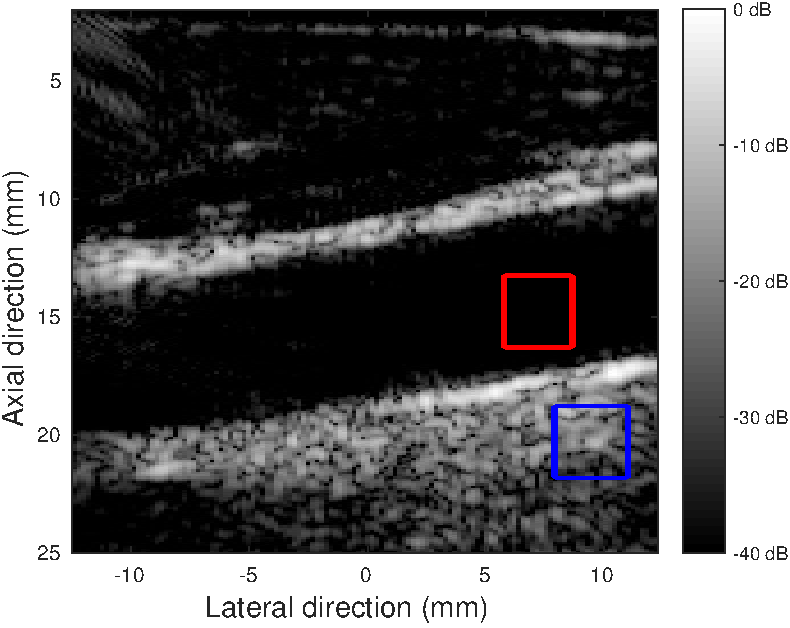
\includegraphics[width=\CarotidFigWidth]{figures/classicalDASCarotid.pdf}} 
\begin{figure*}[htb]
	% Maximum length
	\hfill%
	\subcaptionbox{ }{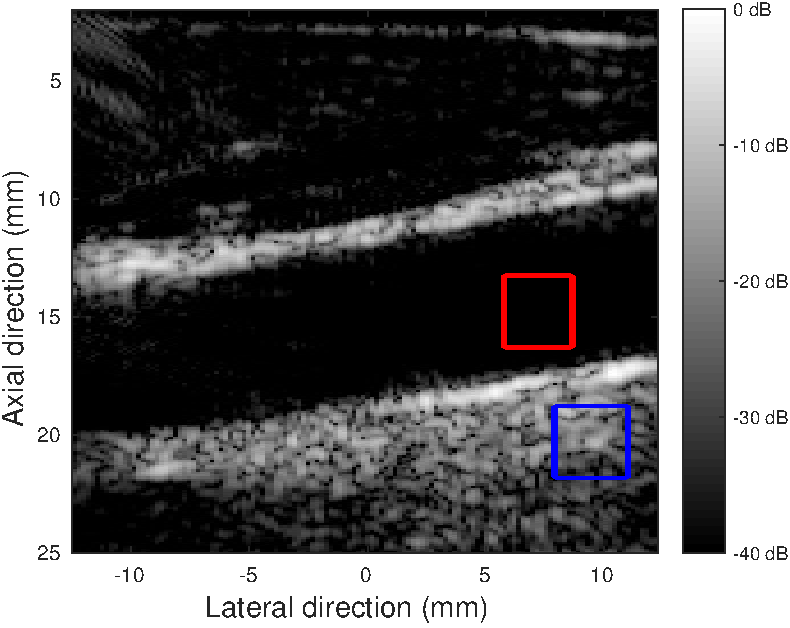
\includegraphics[height=\CarotidFigHeight]{figures/classicalDASCarotid.pdf}}\hfill%
	\subcaptionbox{ }{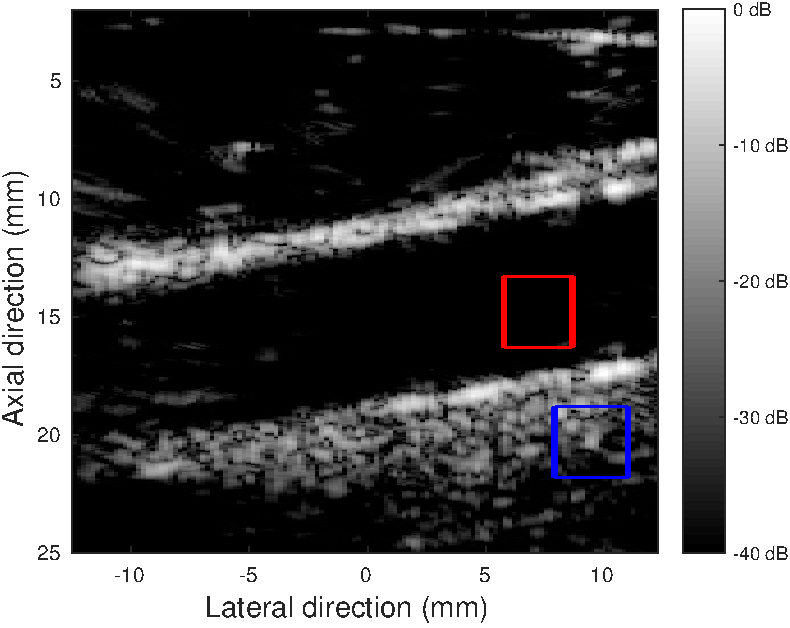
\includegraphics[height=\CarotidFigHeight]{figures/CSCarotid25Beta07.pdf}}\hfill%
	\subcaptionbox{}{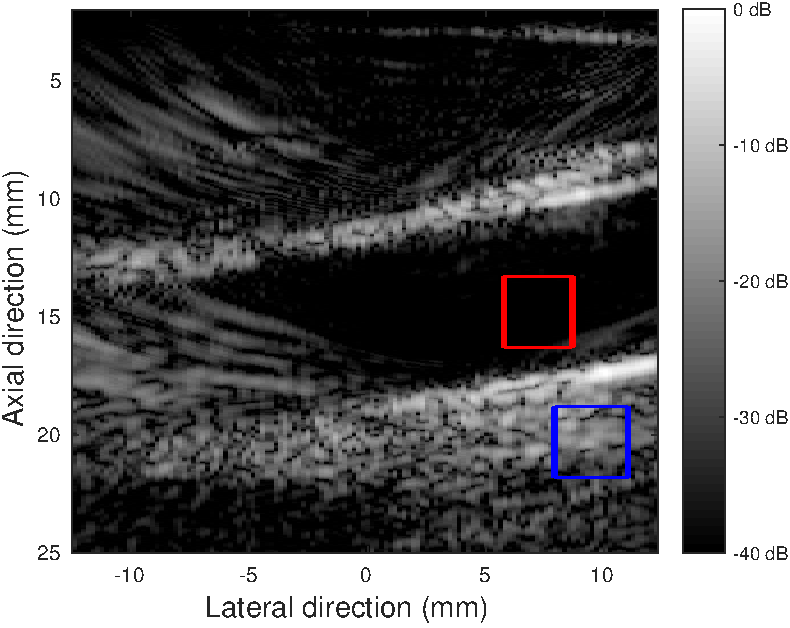
\includegraphics[height=\CarotidFigHeight]{figures/CarotidDASInterp.pdf}}\hfill%
	\caption{B-mode image of an \textit{in vivo} carotid insonified with 5 SPWs and reconstructed with (a) DAS with 128 transducer elements on receive, (b) CB with 32 elements on receive and (c) DAS-interp with 32 elements on receive.}
\end{figure*}
%%% END %%%
\subsection{Diverging wave imaging}
\label{subsec:PW_exp}
A simulation study has been performed to test the framework on DWs. A phantom composed of an 8-\SI{}{\milli\metre} anechoic cyst positioned at \SI{80}{\milli\metre} and embedded in a medium with a high density of scatterers (30 scatterers per resolution cell) is insonified with 3 successive DWs whose corresponding virtual sources are positioned at \SIlist{-5.9;0;5.9}{\milli\metre} in the lateral dimension and at \SI{-2.93}{\milli\metre} in the axial dimension. The probe used in the study mimics a phased-array with 64 transducer elements, a central frequency of \SI{2.7}{\mega\hertz} and a half-wavelength pitch. The generation of simulated raw data is performed using Field~II software~\cite{Jensen1996}.  The element raw data are received with few randomly selected transducer elements spanning the whole aperture. The desired image is reconstructed with both DAS-interp and CB. 
\par The reconstruction methods are compared in terms of contrast-to-noise-ratio (CNR)~\cite{Carrillo_IUS_2015} against the number of transducers selected on receive. B-mode images are also displayed on Figure \ref{fig_DW}. The CNR values, displayed in Figure \ref{fig_CNR}, as well as a visual assessment show that the proposed approach leads to better image reconstruction than classical interpolation.
\settoheight{\CarotidFigHeight}{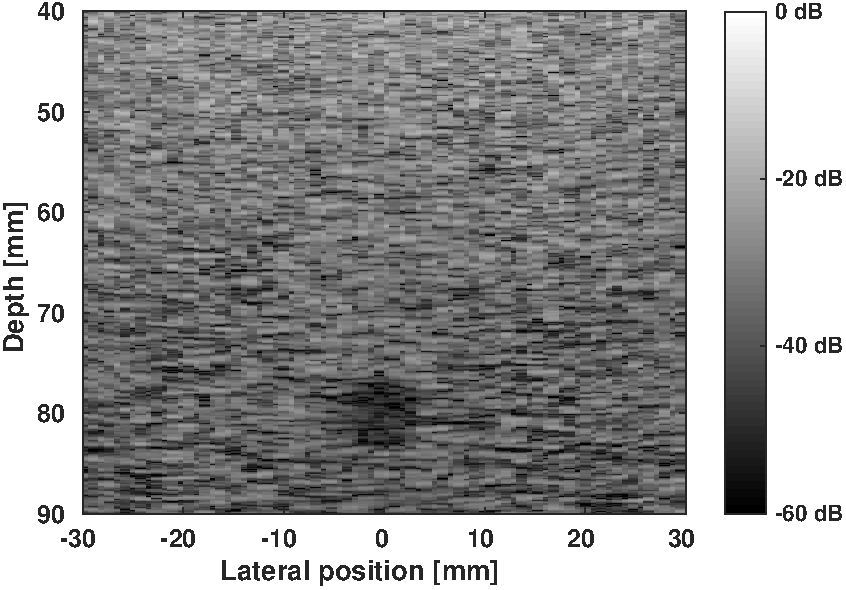
\includegraphics[width=\CarotidFigWidth]{figures/cyst_DW_CS.pdf}} 
%%% FIGURE %%%
\begin{figure*}[htb]
	% Maximum length
	\hfill%
	\subcaptionbox{ }{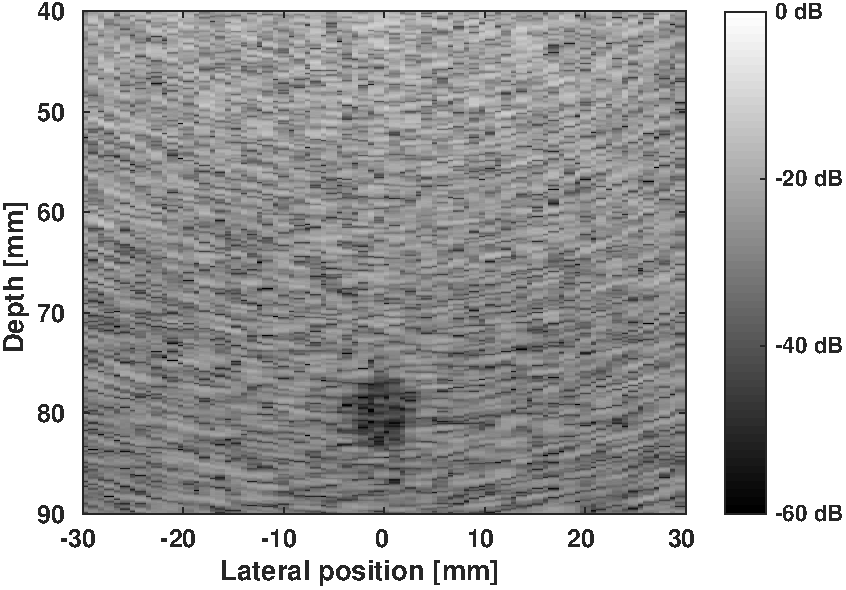
\includegraphics[height=\CarotidFigHeight]{figures/cyst_DW_reference.pdf}}\hfill%
	\subcaptionbox{ }{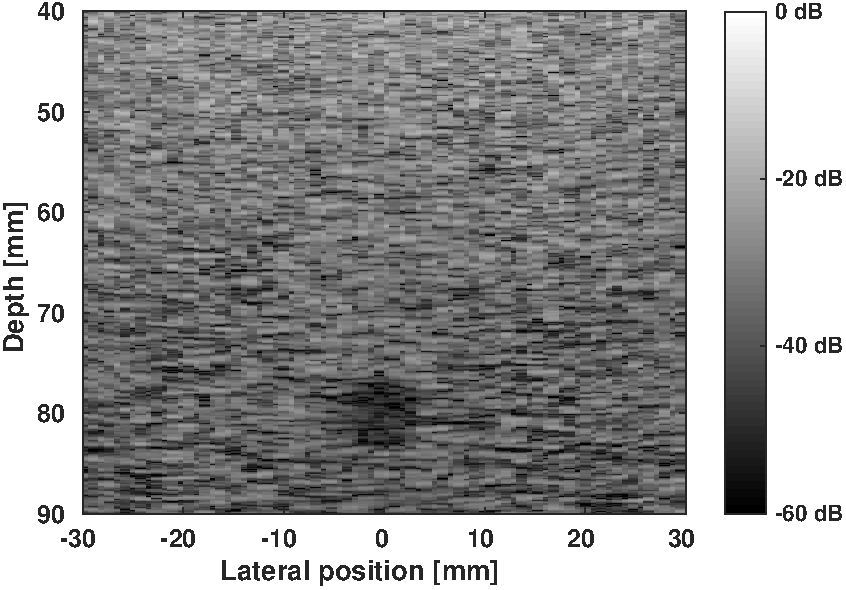
\includegraphics[height=\CarotidFigHeight]{figures/cyst_DW_CS.pdf}}\hfill%
	\subcaptionbox{}{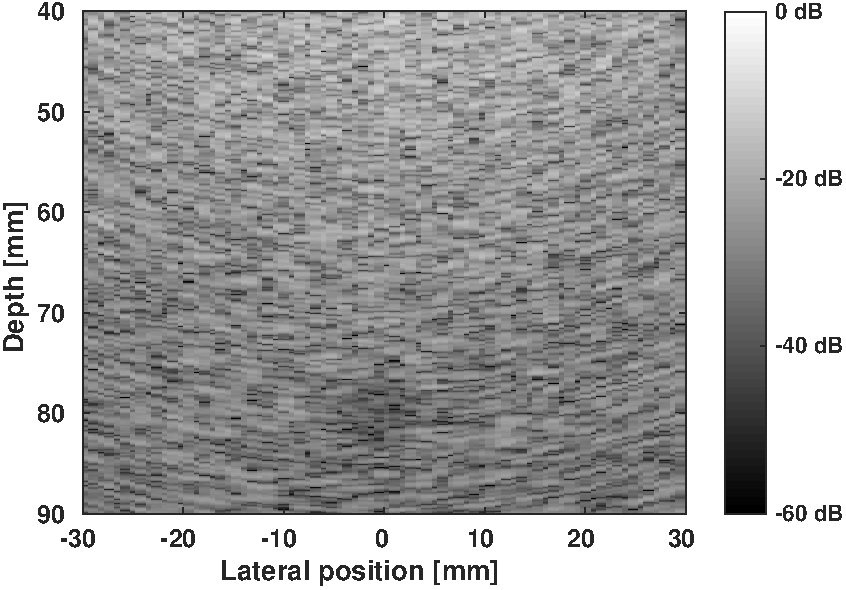
\includegraphics[height=\CarotidFigHeight]{figures/cyst_DW_interp.pdf}}\hfill%
	\caption{B-mode image of a simulated cyst insonified with 3 DWs and reconstructed with (a) DAS with 64 transducer elements on receive, (b) CB with 21 elements on receive and (c) DAS-interp with 21 elements on receive.}
	\label{fig_DW}
\end{figure*}
%%% END OF FIGURE %%%
%%% FIGURE %%%
\begin{figure}[htb]
	\centering
	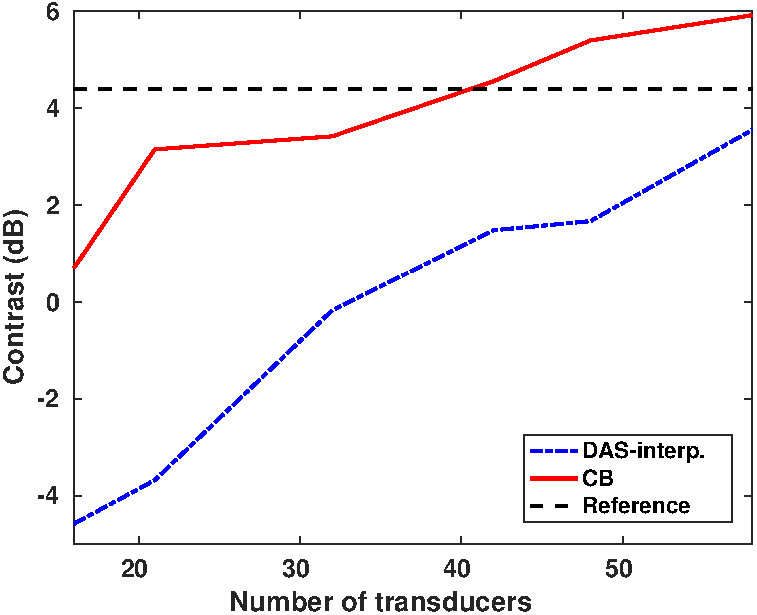
\includegraphics[scale = 0.4]{figures/CNR_DW_IUS2016.pdf}
	\caption{Contrast-to-noise ratio (dB) against the number of transducer elements on receive for DAS-interp (dashed-dot-blue line) and for CB (red-solid line). The dashed-black line represents the contrast measured on the Reference image (DAS with 64 elements).}
	\label{fig_CNR}
\end{figure}
%%% END FIGURE %%%
\section{Conclusion}
\label{sec:Conc}
In this paper, a compressed beamforming framework is presented, which permits to apply CS-based algorithms with a tractable measurement model for both plane-wave- and diverging-wave-coherent compounding as well as for both IQ and RF data. Equipped with an appropriate downsampling scheme, such a framework allows us to fully benefit from the CS-based algorithm in order to recover high quality images from few selected transducer elements.
\section*{Acknowledgements}
This work was supported in part by the UltrasoundToGo RTD project (no. 20NA21 145911), evaluated by the Swiss NSF and funded by Nano-Tera.ch with Swiss Confederation financing. The RF Verasonics generator was cofounded by the FEDER
program, Saint-Etienne Metropole (SME) and Conseil General de la Loire (CG42) within the framework of the SonoCardio-Protection Project leaded by Pr Pierre Croisille.

\bibliographystyle{ieeetr}
\bibliography{IUS2016}

\end{document}


